\chapter{Bevezetés}
\pagenumbering{arabic}
\thispagestyle{empty}

A OpenOffice.org egy teljes körű irodai programcsomag.  Ennek a
programcsomagnak része az OpenOffice.org Calc (továbbiakban
\textbf{\textit{Calc}}), ami egy kiváló táblázatkezelő
program. Segítségével számításokat, matematikai,
pénzügyi elemzéseket végezhetünk, grafikusan
ábrázolhatjuk számadatainkat.

A jelenleg legelterjedtebb táblázatkezelő programmal --  a
Microsoft Excellel --  szemben ez ingyenes, tetszőleges célra
felhasználható szabad szoftver.


\section{A Calc program ablaka}

\begin{figure}[!h]
\begin{center}
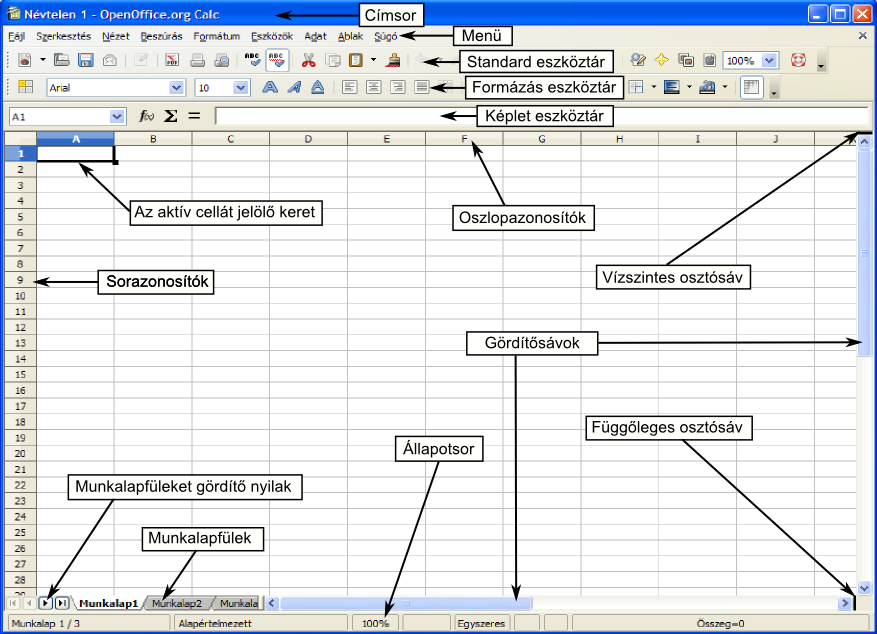
\includegraphics[width=13.999cm]{oocalcv2-img2.png}
\caption{OpenOffice.org Calc ablak}\label{Ablak}
\end{center}
\end{figure}

A \textbf{\textit{Calc}} programot elindítva figyeljük meg
ablakának részeit (\ref{Ablak} ábra). A \textbf{Címsor}ban látjuk a
 dokumentum és a program nevét. Nem mentett dokumentum esetén a
,,Névtelen'' nevet látjuk.  A
címsor alatt a \textbf{Menü} található. Ezekre a menüpontokra
kattintva kategóriákba rendezetten elérhető a program
összes funkciója. A  leggyakrabban használt parancsokat
kiadhatjuk az eszköztárak ikonjai segítségével is.
Alapértelmezés szerint három eszköztárat látunk:
\textbf{Standard}, \textbf{Formázás} és \textbf{Képlet}
eszköztár. A \textbf{Nézet} menüpont \textbf{Eszköztárak}
parancsával több eszköztár is bekapcsolható. Az
 eszköztárak pozíciója megváltoztatható az egér
,,fogd és vidd'' funkciójával, a
bal szélükön látható pontozott oszlopnál megfogva.

Az eszköztárak alatt a táblázatkezelő dokumentumablakát
láthatjuk. Egy 1024 oszlopból és 1048576 sorból álló
táblázatot, ahol az oszlopokat betűkkel (A, B, C, {\dots}, AA,
{\dots}, AMJ), míg a sorokat egész számokkal (1, 2, 3, {\dots},
1048576) jelölik. Ezt a táblázatot Munkalapnak nevezzük. A Calc
induláskor három munkalapot hoz létre automatikusan. Ezek
között a munkalapfülek segítségével válthatunk. A
munkalapfüleken a munkalapok neveit láthatjuk. A fülek
bármelyikén jobb egérgombbal kattintva, a megjelenő
gyorsmenü segítségével átnevezhetjük a munkalapokat,
illetve további munkalapokat hozhatunk létre.

A munkalapfülektől balra a lapfüleket gördítő nyilakat
találjuk. Több munkalap esetén előfordulhat, hogy nem
látjuk mindegyik munkalapfület. Ilyenkor ezekkel a nyilakkal
görgethetjük a munkalapfülek sorát.

A munkalap legkisebb elemét cellának nevezzük. Minden cellának
címe van, ami az oszlop és a sorazonosítóból tevődik
össze. Tehát a munkalap bal felső sarkában az A1-es cella
található, mellette közvetlenül a B1-es.

Az éppen használt munkalapnak mindig van aktív cellája. Ezt a
cellát keret jelöli, és a sor- és az oszlopazonosító,
amelyek metszéspontján az aktív cella található, ki van
emelve.

Az \textbf{Állapotsor} az ablak legalján található. Rajta az
aktuális munkalapra vonatkozó különböző információkat
láthatunk.

Nagyobb táblázatoknál hasznos lehet, hogy a vízszintes és a
függőleges osztósáv segítségével feloszthatjuk a
munkalapot több részre. Így megoldható, hogy egyszerre lássuk
a képernyőn a táblázat két, egymástól sok cellányi
távolságra lévő sorát vagy oszlopát.  


\section{A Súgó használata}

\begin{figure}[!h]
\begin{center}
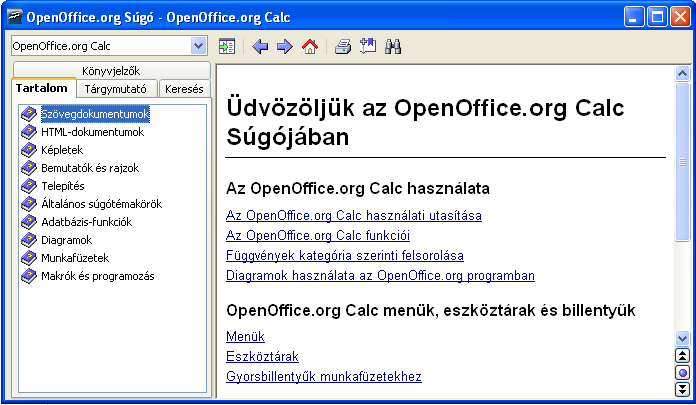
\includegraphics[width=15.999cm]{oocalcv2-img3.png}
\caption{OpenOffice.org Súgó}\label{Súgó}
\end{center}
\end{figure}

A \textit{Calc} programban igen részletes, magyar nyelvű
segítséget jeleníthetünk meg a \textbf{Súgó} menü
\textbf{OpenOffice.org Súgó} parancsával, vagy az F1
funkcióbillentyű lenyomásával. A megjelenő ablakban (\ref{Súgó}
ábra) megtaláljuk a menük, eszköztárak elemeinek
magyarázatát, a függvények kategória szerinti
felsorolását és példákat a használatukhoz, de kereshetünk
a Súgó teljes szövegében is.
A Súgó általunk hasznosnak ítélt oldalait ki is nyomtathatjuk
a \textbf{Nyomtatás\dots} paranccsal,  vagy könyvjelzőt
rendelhetünk az adott súgóoldalhoz.

A Calckal való ismerkedés során nagyon hasznos lehet, hogy a
\textbf{Súgó} menü \textbf{Mi ez?} parancsával a program
ablakának több eleméről tippet kaphatunk. Ilyenkor az egér
mutatója alakot vált, és amire mutatunk vele, arról rövid
magyarázatot olvashatunk a megjelenő szövegdobozban. \Aref{Miez}
ábrán a \textbf{Standard} eszköztár \textbf{Kivágás}
parancsáról megjelenő tippet láthatjuk.
\begin{figure}[!h]
\begin{center}
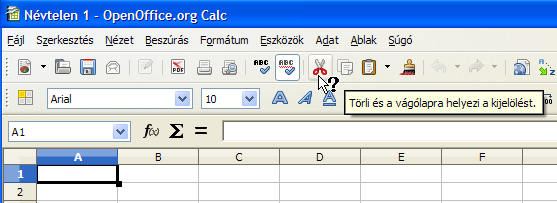
\includegraphics[width=14.736cm]{oocalcv2-img4.png}
\caption{OpenOffice.org Mi ez?}\label{Miez}
\end{center}
\end{figure}
